\documentclass[border=3mm]{standalone}

\usepackage{tikz}
\usetikzlibrary{arrows,shapes.gates.logic.US,shapes.gates.logic.IEC,calc}
\begin{document}
\thispagestyle{empty}
\tikzstyle{branch}=[fill,shape=circle,minimum size=5pt,inner sep=0pt]
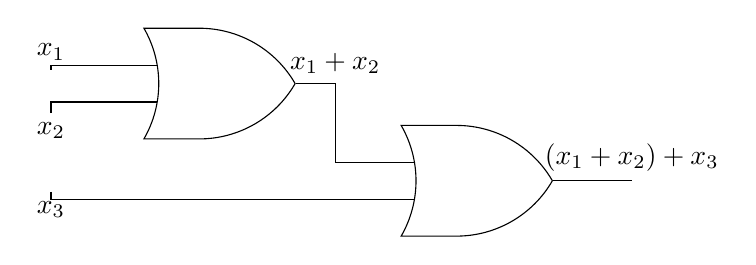
\begin{tikzpicture}[label distance=2mm]

    \node (x1) at (0,0) {$x_1$};
    \node (x2) at (0,-1) {$x_2$};
    \node (x3) at (0,-2) {$x_3$};

    \node[or gate US, draw, logic gate inputs=nn, minimum size=40pt] at (2,-0.4) (Or1) {};
    \node[or gate US, draw, logic gate inputs=nn, anchor=input 1, minimum size=40pt] at ($(Or1.output)+(1.5,-1)$) (Or2)  {};

    \draw (x1) |- (Or1.input 1);
    \draw (x2) |- (Or1.input 2);
    \draw (x3) |- (Or2.input 2) ;
    %\draw (Or1.output |- Or2.input 1) node[above] {};
    \draw (Or1.output) -- ([xshift=0.5cm]Or1.output)node[above] {$x_1 + x_2$} |- (Or2.input 1)  ;
    \draw (Or2.output) -- ([xshift=1cm]Or2.output) node[above] {$(x_1 + x_2) + x_3$};
\end{tikzpicture}
\end{document} 
